\documentclass{phyasgn}\usepackage{nag}
\phyasgn{classname=纳电子器件导论课程论文}
\usepackage[backend=bibtex,bibstyle=gb7714-2015,citestyle=gb7714-2015]{biblatex}
\setlength{\bibitemsep}{3bp}
\addbibresource{ref.bib}
\renewcommand*{\bibfont}{\zihao{5}\linespread{1.27}\selectfont}
%\usepackage{background}
%\backgroundsetup{scale=1,angle=0,opacity=1,contents={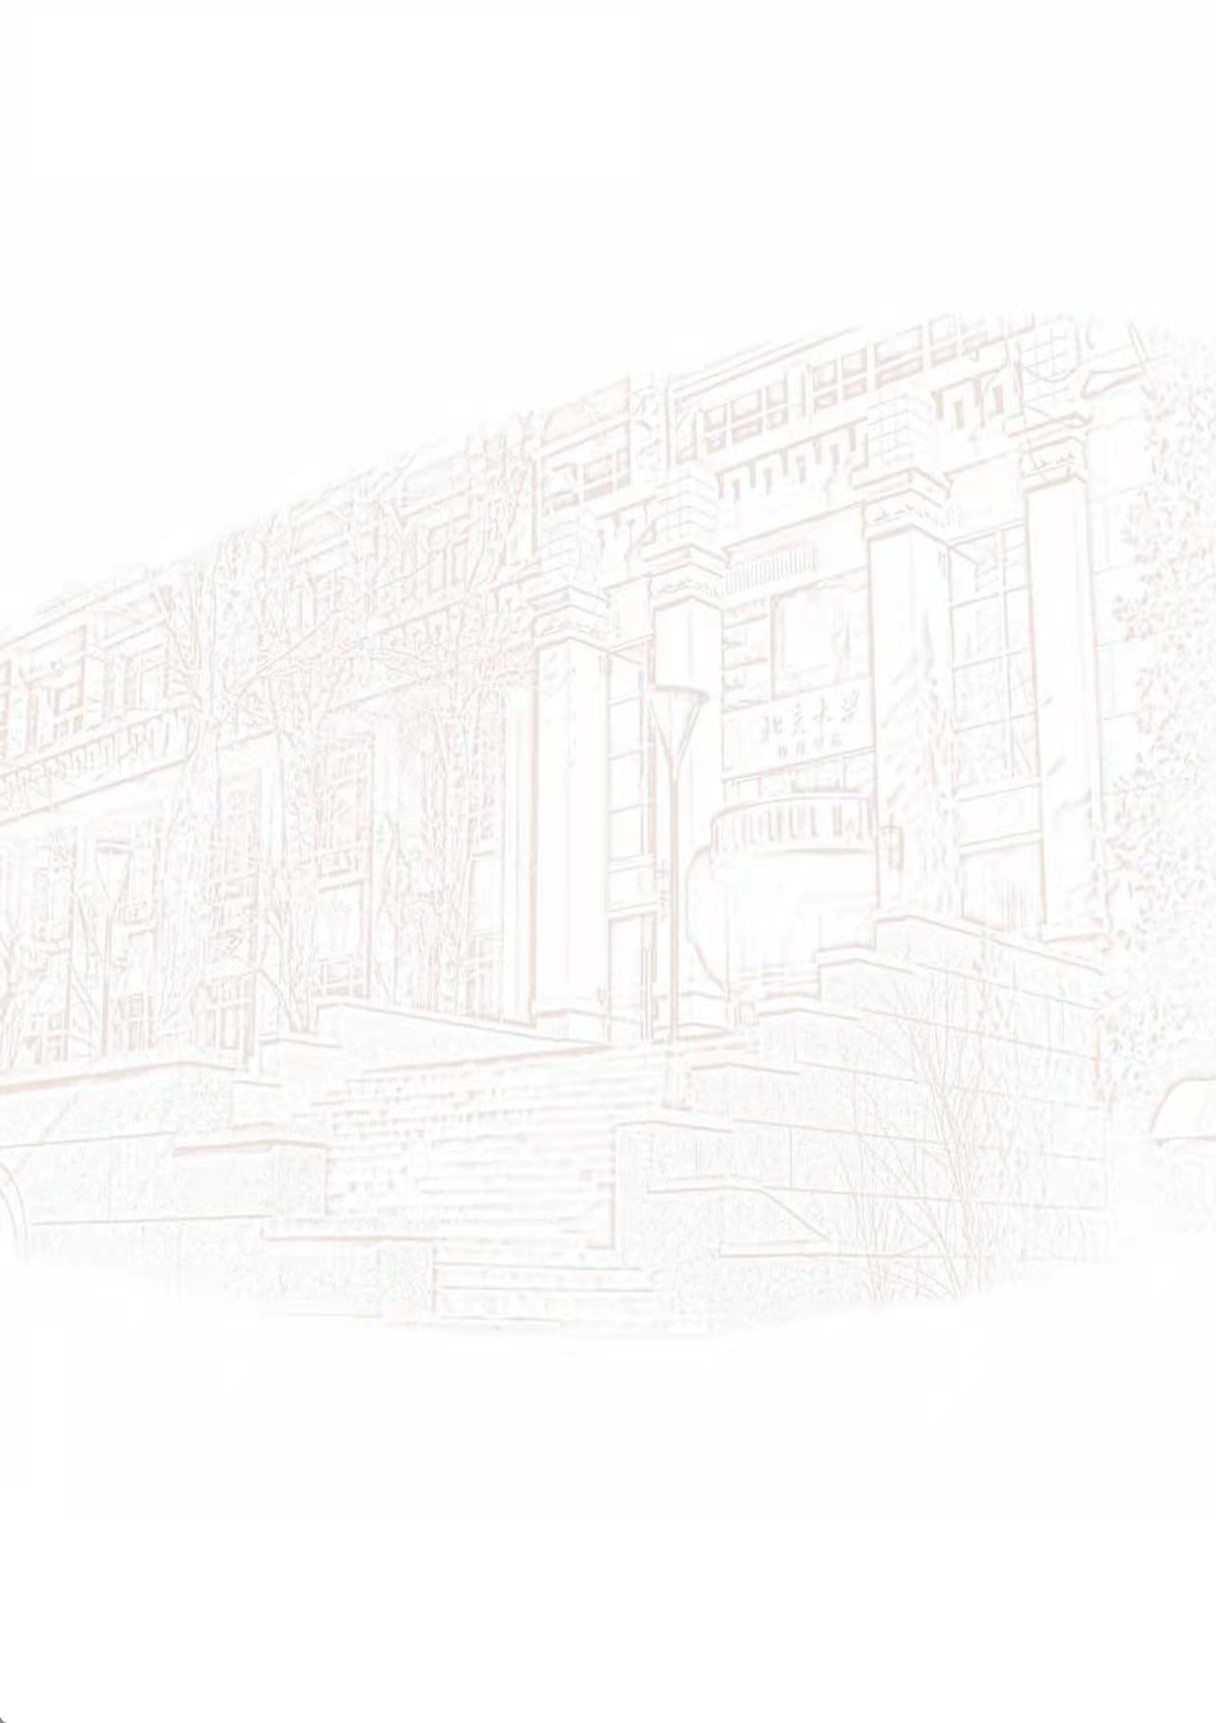
\includegraphics[width=\paperwidth, height=\paperwidth, keepaspectratio]{pic/phy.jpg}}}
%\ctexset{punct=kaiming}
\setCJKmainfont[ItalicFont=FZKTK.TTF,BoldFont=FZXBSK.TTF]{FZSSK.TTF}
\setCJKsansfont[BoldFont=FZHTK.TTF]{FZXH1K.TTF}
\setCJKmonofont[ItalicFont=FZKTK.TTF]{FZFSK.TTF}
\newCJKfontfamily\FZSS{FZSSK.TTF}
\newCJKfontfamily\FZKT{FZKTK.TTF}
\newCJKfontfamily\FZFS{FZFSK.TTF}
\newCJKfontfamily\FZHT{FZHTK.TTF}
\setmainfont{TeX Gyre Termes}
\setsansfont{TeX Gyre Heros}[Scale=MatchLowercase]
\setmonofont{Ubuntu Mono}%[Scale=MatchLowercase]
\newfontfamily\lm{Latin Modern Roman}
\usepackage{unicode-math}
\setmathfont{TeX Gyre Termes Math}

\newcommand\pkg[1]{\textsf{#1}}
\newenvironment{csop}{\vskip\topsep\noindent\hspace{2em}\ttfamily\small\ignorespaces}{\vskip\topsep\par}
\usepackage{float}
\usepackage{booktabs,metalogo,siunitx,marginnote,manfnt,url}
\usepackage[unicode]{hyperref}
\hypersetup{pdfstartview=XYZ,hidelinks,pdfcreator=XeTeX Output,pdfauthor=吴熙楠,
pdftitle=phyasgn文档类}
\usepackage{geometry,fancyhdr}
\geometry{left=3cm,right=3cm,marginparwidth=4em}
\fancyhead[L]
{\begin{tabular}[b]{@{}l@{}}
  \hyperref{https://www.pku.edu.cn/}{}{}{
\includegraphics[height=2.12em]{pic/pkulogo.jpg}}
\end{tabular}}
\fancyhead[C]
{\begin{tabular}[b]{@{}c@{}}
  \large 
  基于磁矩探测石墨烯的Fe$^{3+}$与Cu$^{2+}$分布
  \\[-2pt]
  {\scriptsize 姓名:~吴熙楠\quad 学号:~1900011413}
\end{tabular}
}

\usepackage{shortvrb,fancyvrb}
\MakeShortVerb|
\fvset{xleftmargin=2em,fontsize=\small}
\makeatletter
\ifx\l@nohyphenation\undefined
  \newlanguage\l@nohyphenation
\fi
\DeclareRobustCommand\meta[1]{%
  \ensuremath\langle
  \ifmmode \expandafter \nfss@text \fi
  {%
    \rmfamily\itshape
    \edef\meta@hyphen@restore
    {\hyphenchar\the\font\the\hyphenchar\font}%
  \hyphenchar\font\m@ne
  \language\l@nohyphenation
  #1\/%
  \meta@hyphen@restore
  }\ensuremath\rangle
}
\makeatother

\def\phyasgn{\pkg{phyasgn}}
\def\version{0.2 $\upbeta$}

\title{
  {基于磁矩探测石墨烯的Fe$^{3+}$与Cu$^{2+}$分布}\\[-8pt]
  {\normalsize ——纳电子器件课程论文}
}
\author{吴熙楠}
\date{\today}
\begin{document}
\maketitle

\begin{abstract}
利用石墨烯制备场效应晶体管时,通常采用湿法将石墨烯转移至SiO$_2$表面,由于在此过程中需要浸泡在FeCl$_3$溶液中,因此沟道上会不可避免地残留Fe$^{3+}$和Cu$^{2+}$。在本文中,将利用Fe$^{3+}$和Cu$^{2+}$掺杂石墨烯会带来磁矩的这个原理来设计一种能超灵敏、高分辨探测沟道内Fe$^{3+}$和Cu$^{2+}$的方法。
\end{abstract}

\tableofcontents

\section{引言}
\par 利用石墨烯制备场效应晶体管时,通常采用湿法将石墨烯转移至SiO$_2$表面,由于在此过程中需要浸泡在FeCl$_3$溶液中,因此沟道上会不可避免地残留Fe$^{3+}$和Cu$^{2+}$。同时除了残留的Fe$^{3+}$和Cu$^{2+}$外,沟道本身也有离子掺杂,如果说我们认为离子是均匀掺杂且数量较多,那么这些沟道内衬底本身自带的离子可以认为是一个背景噪声分布,只要我们选取合适的零点就可以消去,我们可以根据它们所带电荷数的不同测定沟道的电荷分布从而可以比较容易地得出这些离子的分布情况。但是我们的这个假设是不合适的,很明显我们很难保证衬底的离子分布均匀,这也就会导致我们通过电荷测量分布的错误,同时由于衬底本身存在一定的杂质离子,我们也不能通过石墨烯弹道输运变化来判断Fe$^{3+}$与Cu$^{2+}$的分布。由于我们知道在如Fe和Cu这样存在3d轨道与4d轨道的过渡金属掺杂到石墨烯里的时候,会使得石墨烯出现局域电子态,并出现顺磁特性\cite{sadki2019spontaneous},我将考虑从石墨烯的磁性质出发探测沟道内的离子分布(假设沟道内的杂质离子不会使得石墨烯出现多余的磁矩,即非过渡金属离子)。
\section{想法内容}
\par 因为我们知道在如Fe和Cu这样存在3d轨道与4d轨道的过渡金属掺杂到石墨烯里的时候,掺杂的部分会使得石墨烯出现局域电子态,并出现顺磁特性(当然我们也可以测量在费米面附近的电子态密度,如果有Fe$^{3+}$或Cu$^{2+}$,那么那处的电子态密度会出现一个峰值)\cite{sadki2019spontaneous}。本身而言我们可以利用STM或者MFM来将器件的石墨烯表面扫描一遍就能测出表面的磁感应强度分布,但是由于我们制备的石墨烯不是完好无缺的(呈现抗磁性),如果石墨烯表面存在空位缺陷的话,这些缺陷位置就会出现顺磁性,并在单位空位形成$1.12\mu_{B}\sim 1.53\mu_{B}$的磁矩\cite{haffad2018effect,septya2021electronic},因此我们并不能区分这到底是Fe$^{3+}$,Cu$^{2+}$还是空位引起的磁矩变化,所以我们需要消除空位的影响。
\par 为了消除空位带来磁矩的影响,我们需要选择可控的且可以填补空位的表面钝化的方式。为此我们选择用H原子进行钝化(H原子掺杂对石墨烯磁性的影响在多个文献上均有报道\cite{gonzalez2016atomic,haffad2018effect,ray2018electronic}),在掺杂过后原空位处会出现约$1\mu_{B}$的磁矩大小,而被H原子吸附的C原子周围存在$0.1\mu_{B}$的磁矩\cite{septya2021electronic},而文献报道出现磁矩的原因是两个H原子被化学吸附在同一个碳亚晶格上,即自旋极化态固定在一个碳亚晶格上与H原子吸附的亚晶格互补,而如果我们使用STM将其中一个H原子横向移动到相反的亚晶格上,形成AB二聚体构型,这个构型就是非磁性的\cite{gonzalez2016atomic}。但是对于Fe$^{3+}$与Cu$^{2+}$而言,它们的铁磁性质具有磁滞回线,周围磁场变为0了还有剩余磁矩,因此我们仍然可以使用STM或MFM探测到其磁矩大小。
\par 同时为了区分出Fe$^{3+}$与Cu$^{2+}$的分布,我们在上一步明确石墨烯表面各区域的磁矩分布过后,我们可以使用STM测量出费米面附近不同区域处的电子态密度,由于Fe$^{3+}$与Cu$^{2+}$掺杂下石墨烯电子态密度在费米面处的峰位不同\cite{sadki2019spontaneous},以及Fe$^{3+}$与Cu$^{2+}$掺杂石墨烯情况下引入的磁矩不同,将二者进行对比同时结合单独Fe$^{3+}$与Cu$^{2+}$掺杂下产生的磁矩大小,我们即可得出Fe$^{3+}$与Cu$^{2+}$分别的分布。(或者我们可以使用X射线光电子能谱分析样品的掺杂Fe$^{3+}$与Cu$^{2+}$的量,同时与之前测出来的石墨烯样品表面磁矩分布对比即可得出Fe$^{3+}$与Cu$^{2+}$的分布)
\section{拟实施的途径或方案}
\par 首先我们需要对石墨烯进行氢等离子体处理,使得H均匀吸附在石墨烯表面上,这时整个石墨烯器件都会带有磁性,但是此时存在Fe$^{3+}$与Cu$^{2+}$的地方与石墨烯器件表面其余地方的磁矩不同。然后我们使用STM将H原子全部横向移动到与其相反的亚晶格上面去,这样使得H原子全部实现AB二聚体构型,不显磁性。此时我们可以使用STM或者MFM对样品表面进行一个遍历扫描可以测出表面的磁矩或者磁感应强度的整体分布,这就是由于Fe$^{3+}$与Cu$^{2+}$的分布引起的。之后我们再利用STM测出样品表面不同位置费米面附近的电子态密度分布,与单独Fe$^{3+}$和Cu$^{2+}$掺杂时的电子态密度对比就可以得出Fe$^{3+}$与Cu$^{2+}$在沟道内的分布。(当然这是建立在Fe$^{3+}$与Cu$^{2+}$对于电子局域态密度方面互不影响的情况下,即Fe$^{3+}$与Cu$^{2+}$在石墨烯中不存在强的相互作用,如果其相互作用不能忽视,我们就只能使用X射线光电子能谱分析得出Fe$^{3+}$与Cu$^{2+}$的元素分布情况,再与磁矩或者磁感应强度分布情况对比得出Fe$^{3+}$与Cu$^{2+}$在沟道内的分布)
\section{想法基于的原理}
\par 由文献报道中第一性原理的计算\cite{sadki2019spontaneous},可以得到对于有3d轨道的过渡金属元素掺杂下,掺杂位置存在的最大磁矩大小为Mn产生的$3.57\mu_{B}$,最小为Co产生的$1.52\mu_{B}$,因此Fe与Cu掺杂应该介于$1.52\mu_{B}\sim 3.57\mu_{B}$之间。
\par 在石墨烯上由于缺陷会导致其出现局域态,从而产生磁性。比如吸附原子会破坏石墨烯的对称性,在吸附原子周围产生自旋极化态(如下图),同理空位也会破坏石墨烯的亚晶格的对称性,从而产生磁性准局域态,从而产生磁性\cite{ray2018electronic}。
\begin{figure}[H]
	\centering
	\hspace{2em}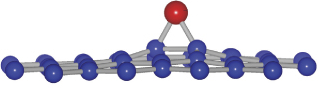
\includegraphics[width=.45\linewidth]{pic/3.jpg}
	\caption{石墨烯吸附原子示意图\cite{ray2018electronic}
	}
\end{figure}
\par 将H原子横向移动到相反亚晶格上,将会形成AB二聚体从而变为非磁性:
\begin{figure}[H]
	\centering
	\hspace{2em}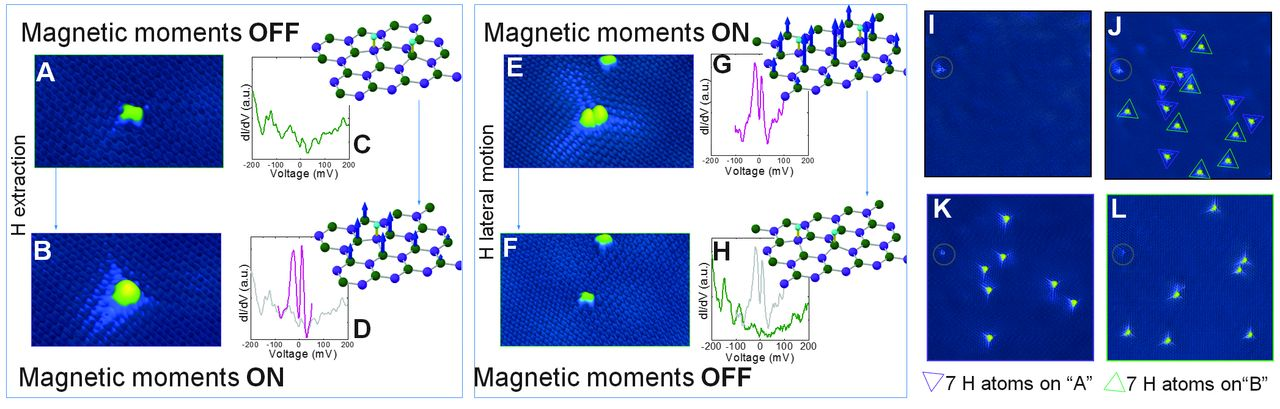
\includegraphics[width=.8\linewidth]{pic/1.jpeg}
	\caption{STM对石墨烯局部磁矩的操纵\cite{gonzalez2016atomic}
	}
\end{figure}
\par 不同的过渡金属元素掺杂会导致费米面附近的局域电子态密度发生变化:
\begin{figure}[H]
	\centering
	\hspace{2em}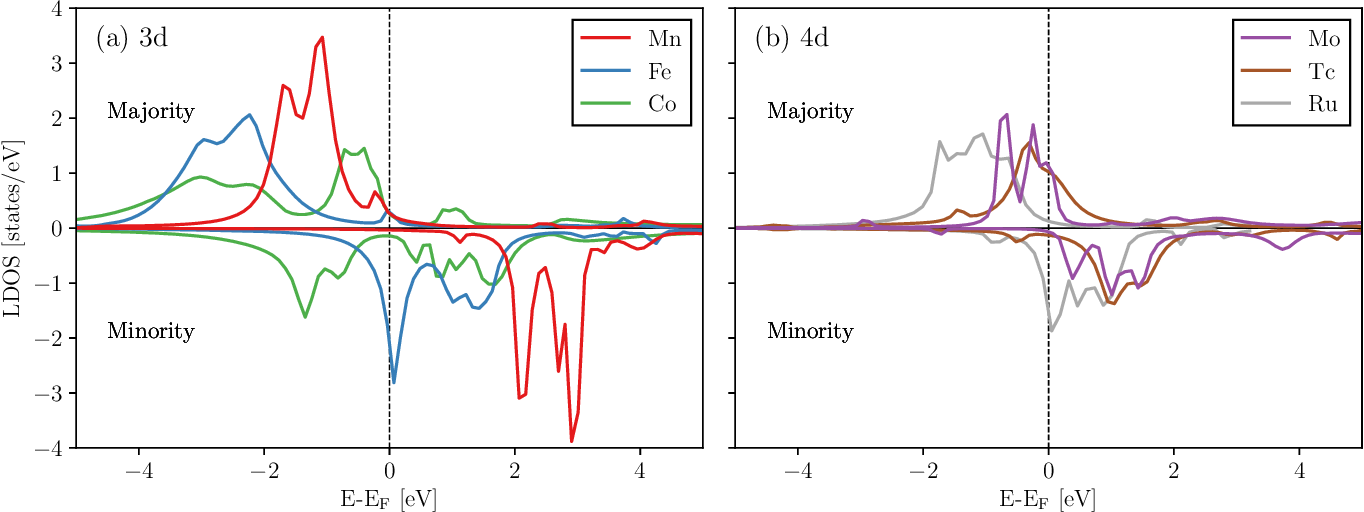
\includegraphics[width=.75\linewidth]{pic/2.png}
	\caption{(a)3d和(b)4d吸附原子时的局部态密度\cite{sadki2019spontaneous}
	}
\end{figure}
\section{期待的结果}
\par 如果一切能如上所述顺利进行的话,我们应该可以得到磁矩或者磁感应强度在沟道内的分布(结合单独Fe$^{3+}$与Cu$^{2+}$掺杂时的磁矩大小),并且得到清晰的电子态密度的分布图,然后我们就能通过两个分布的对比得到Fe$^{3+}$与Cu$^{2+}$在沟道内的分布。(或者使用X射线光电子能谱分析结合整体的磁矩大小分布以及单独的Fe$^{3+}$与Cu$^{2+}$掺杂后磁矩大小,我们也能得到Fe$^{3+}$与Cu$^{2+}$在沟道内的分布)
\section{总结与展望}
\par 总的来说,这种方法步骤简单,操作也不复杂(但是使用STM横向移动H原子可能会稍微繁琐一些),物理图像清楚,而且由于STM,MFM等的操作都是原子级别的操作,因此我们也能满足超灵敏、高分辨探测的要求。但是由于Fe$^{3+}$与Cu$^{2+}$都是过渡金属元素,因此其电子云的结构非常复杂,如果是原子级别距离很近,那Fe$^{3+}$与Cu$^{2+}$的3d轨道电子云将会重叠很大,对局域态密度的影响很大,那么就不能使用电子态密度对比来得出Fe$^{3+}$与Cu$^{2+}$分别出来的分布,我们就需要使用X射线光电子能谱分析来辅助探测。但X射线光电子能谱分析虽然也很灵敏,但毕竟X射线照射下对于石墨烯制成的场效应管的性能会有不小的影响。
\par 因此,我们以后在制备样品(不仅是石墨烯样品)的时候,保证样品无杂质是非常重要的,在这方面,机械剥离石墨烯虽然很难得到大面积石墨烯,但是在保证石墨烯的纯净度上还是非常有优势的。
\section{致谢}
\par 感谢傅老师一学期以来对于纳电子器件方面知识的传授,我从这门课里面学到了很多,知识量非常庞大,同时也感受到了傅老师的教学热情与精心布置的作业,培养了我们独立思考的能力,尤其是最后这个期末报告锻炼了我们独立解决问题的能力,以后如果要从事纳电子器件尤其是石墨烯与碳纳米管方面的工作相信也会更加的得心应手吧。
\printbibliography[heading=bibintoc]
\end{document}